\begin{frame}
	\frametitle{Interaktion Hydrosphäre, Kryosphäre und Atmosphäre}
	\begin{figure}
		\centering
		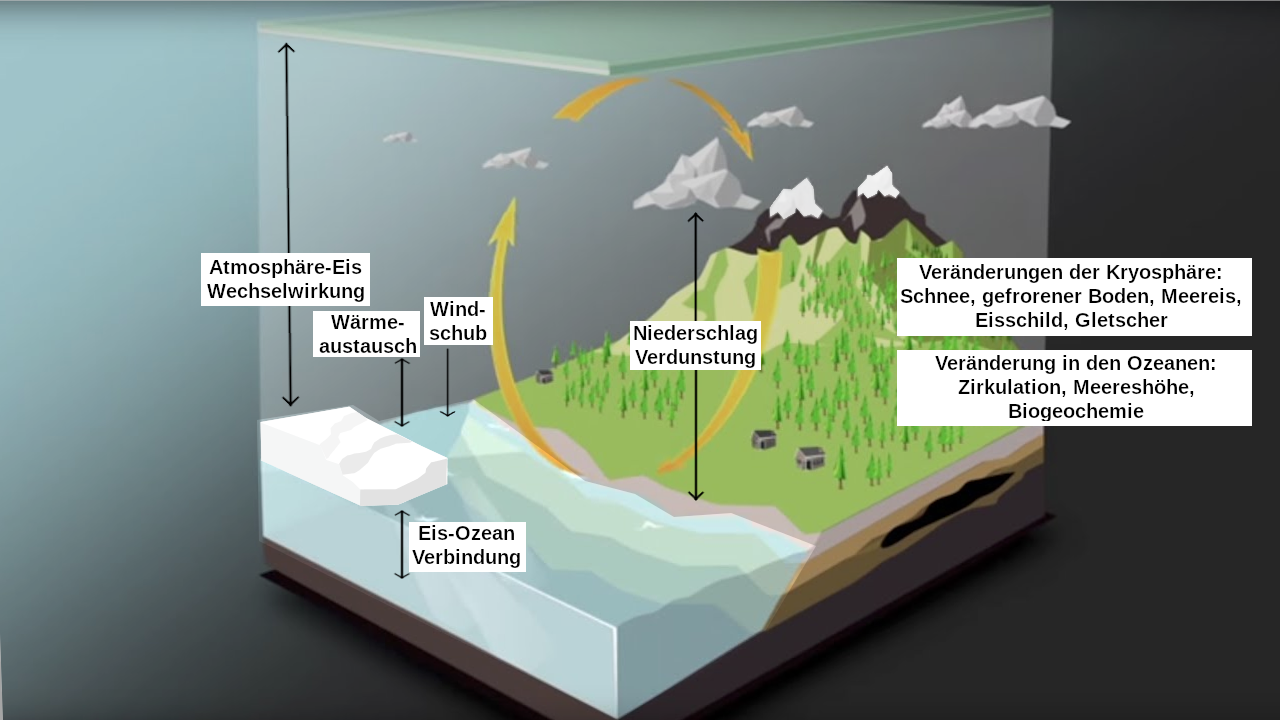
\includegraphics{bilder/WMO_Cycles_factors_waterAndIce.png}
		\caption{Interaktion Hydrosphäre, Kryosphäre und Atmosphäre}
	\end{figure}

	\note{
		\begin{itemize}
			\item[] links an den Pfeilen sind die Wechselwirkungen notiert - z.B. Eis-Ozean-Verbindung (Konvektion)
			\item[] rechts sieht man die allgemeinen Elemente der Komponenten Hydrosphäre und Kryosphäre
			\item[] diese Elemente hängen offensichtlich zusammen und bedingen sich gegenseitig
		\end{itemize}
	}
\end{frame}
